% Page: Studies, data, and evidence
% da-01-studies-and-data.qmd
% The smoking comparison on that page is observational: diet and income can
% differ between the groups of mothers and can also move the sons' heights.
% The blood-pressure trial assigns the drug at random, so age, diet and
% fitness are not a route into the treatment.
\documentclass[border=6pt]{standalone}
\usepackage[T1]{fontenc}
\usepackage{lmodern}
\usepackage{amsmath}
\usepackage{tikz}
\usetikzlibrary{arrows.meta,positioning}
\definecolor{ink}{HTML}{1F2430}
\definecolor{statblue}{HTML}{174A7E}
\definecolor{accent}{HTML}{9C4A32}
\definecolor{grey}{HTML}{5E6A75}
\begin{document}
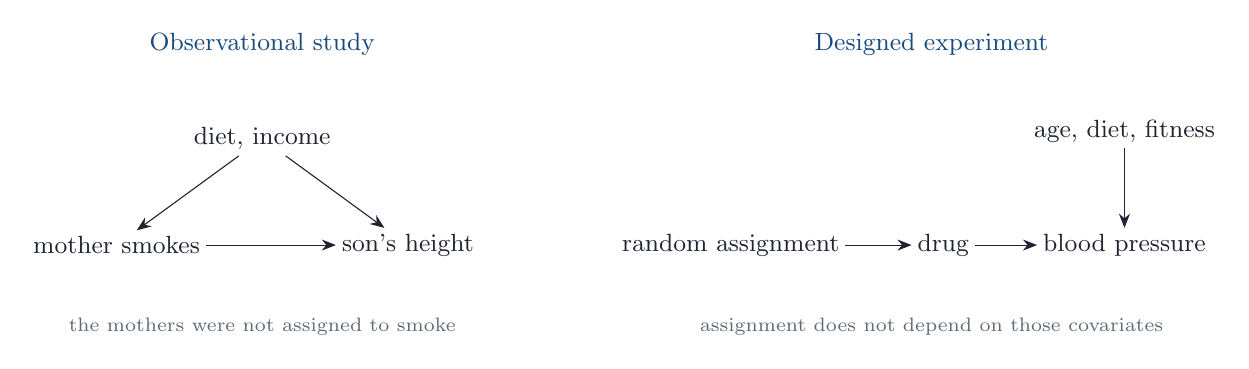
\begin{tikzpicture}[
  font=\small,
  every node/.style={text=ink, inner sep=2pt},
  arr/.style={-{Stealth[length=1.8mm,width=1.4mm]}, ink, thin},
  lab/.style={font=\small, statblue},
]
  % Observational study
  \node[lab] (h1) at (0,2.55) {Observational study};
  \node (diet) at (0,1.35) {diet, income};
  \node (smoke) at (-1.85,0) {mother smokes};
  \node (height) at (1.85,0) {son's height};
  \draw[arr] (diet) -- (smoke);
  \draw[arr] (diet) -- (height);
  \draw[arr] (smoke) -- (height);
  \node[font=\scriptsize, grey, align=center, anchor=north] at (0,-0.85)
    {the mothers were not assigned to smoke};

  % Designed experiment
  \begin{scope}[xshift=8.1cm]
    \node[lab] at (0.4,2.55) {Designed experiment};
    \node (asg) at (-2.15,0) {random assignment};
    \node (drug) at (0.55,0) {drug};
    \node (bp) at (2.85,0) {blood pressure};
    \node (cov) at (2.85,1.45) {age, diet, fitness};
    \draw[arr] (asg) -- (drug);
    \draw[arr] (drug) -- (bp);
    \draw[arr] (cov) -- (bp);
    \node[font=\scriptsize, grey, align=center, anchor=north] at (0.4,-0.85)
      {assignment does not depend on those covariates};
  \end{scope}
\end{tikzpicture}
\end{document}
